\documentclass{sigchi}
\usepackage{float}

% Use this section to set the ACM copyright statement (e.g. for
% preprints).  Consult the conference website for the camera-ready
% copyright statement.

% Copyright
%\CopyrightYear{2020}
%\setcopyright{acmcopyright}
%\setcopyright{acmlicensed}
%\setcopyright{rightsretained}
%\setcopyright{usgov}
%\setcopyright{usgovmixed}
%\setcopyright{cagov}
%\setcopyright{cagovmixed}
% DOI
%\doi{https://doi.org/10.1145/3313831.XXXXXXX}
% ISBN
%\isbn{978-1-4503-6708-0/20/04}
%Conference
%\conferenceinfo{CHI'20,}{April  25--30, 2020, Honolulu, HI, USA}
%Price
%\acmPrice{\$15.00}

% Use this command to override the default ACM copyright statement
% (e.g. for preprints).  Consult the conference website for the
% camera-ready copyright statement.

%% HOW TO OVERRIDE THE DEFAULT COPYRIGHT STRIP --
%% Please note you need to make sure the copy for your specific
%% license is used here!
% \toappear{
% Permission to make digital or hard copies of all or part of this work
% for personal or classroom use is granted without fee provided that
% copies are not made or distributed for profit or commercial advantage
% and that copies bear this notice and the full citation on the first
% page. Copyrights for components of this work owned by others than ACM
% must be honored. Abstracting with credit is permitted. To copy
% otherwise, or republish, to post on servers or to redistribute to
% lists, requires prior specific permission and/or a fee. Request
% permissions from \href{mailto:Permissions@acm.org}{Permissions@acm.org}. \\
% \emph{CHI '16},  May 07--12, 2016, San Jose, CA, USA \\
% ACM xxx-x-xxxx-xxxx-x/xx/xx\ldots \$15.00 \\
% DOI: \url{http://dx.doi.org/xx.xxxx/xxxxxxx.xxxxxxx}
% }

% Arabic page numbers for submission.  Remove this line to eliminate
% page numbers for the camera ready copy
% \pagenumbering{arabic}

% Load basic packages
\usepackage{balance}       % to better equalize the last page
\usepackage{graphics}      % for EPS, load graphicx instead 
\usepackage[T1]{fontenc}   % for umlauts and other diaeresis
\usepackage{txfonts}
\usepackage{mathptmx}
\usepackage[pdflang={en-US},pdftex]{hyperref}
\usepackage{color}
\usepackage{booktabs}
\usepackage{textcomp}

% Some optional stuff you might like/need.
\usepackage{microtype}        % Improved Tracking and Kerning
% \usepackage[all]{hypcap}    % Fixes bug in hyperref caption linking
\usepackage{ccicons}          % Cite your images correctly!
% \usepackage[utf8]{inputenc} % for a UTF8 editor only

% If you want to use todo notes, marginpars etc. during creation of
% your draft document, you have to enable the "chi_draft" option for
% the document class. To do this, change the very first line to:
% "\documentclass[chi_draft]{sigchi}". You can then place todo notes
% by using the "\todo{...}"  command. Make sure to disable the draft
% option again before submitting your final document.
%\usepackage{todonotes}

% Paper metadata (use plain text, for PDF inclusion and later
% re-using, if desired).  Use \emtpyauthor when submitting for review
% so you remain anonymous.
\def\plaintitle{Investigating Fundamental Machine Learning Models}
\def\plainauthor{First Author, Second Author, Third Author,
  Fourth Author, Fifth Author, Sixth Author}
\def\emptyauthor{}
\def\plainkeywords{Authors' choice; of terms; separated; by
  semicolons; include commas, within terms only; this section is required.}
\def\plaingeneralterms{Documentation, Standardization}

% llt: Define a global style for URLs, rather that the default one
\makeatletter
\def\url@leostyle{%
  \@ifundefined{selectfont}{
    \def\UrlFont{\sf}
  }{
    \def\UrlFont{\small\bf\ttfamily}
  }}
\makeatother
\urlstyle{leo}

% To make various LaTeX processors do the right thing with page size.
\def\pprw{8.5in}
\def\pprh{11in}
\special{papersize=\pprw,\pprh}
\setlength{\paperwidth}{\pprw}
\setlength{\paperheight}{\pprh}
\setlength{\pdfpagewidth}{\pprw}
\setlength{\pdfpageheight}{\pprh}

% Make sure hyperref comes last of your loaded packages, to give it a
% fighting chance of not being over-written, since its job is to
% redefine many LaTeX commands.
\definecolor{linkColor}{RGB}{6,125,233}
\hypersetup{%
  pdftitle={\plaintitle},
% Use \plainauthor for final version.
%  pdfauthor={\plainauthor},
  pdfauthor={\emptyauthor},
  pdfkeywords={\plainkeywords},
  pdfdisplaydoctitle=true, % For Accessibility
  bookmarksnumbered,
  pdfstartview={FitH},
  colorlinks,
  citecolor=black,
  filecolor=black,
  linkcolor=black,
  urlcolor=linkColor,
  breaklinks=true,
  hypertexnames=false
}

% create a shortcut to typeset table headings
% \newcommand\tabhead[1]{\small\textbf{#1}}

% End of preamble. Here it comes the document.
\begin{document}

\title{\plaintitle}

\numberofauthors{1}
\author{%
  \alignauthor{Kenny Oseleononmen\\
    \affaddr{Stanford University}\\
    \email{kenny1g@stanford.edu}}\\
}

\maketitle
\section{Introduction}
This paper uses the problem of predicting whether a user will like a restaurant to explore and understand various fundamental machine learning algorithms, namely Logistic Regression, Naive Bayes and Decision Trees.
\section{Dataset and Features}
The origins of the dataset being used is the Yelp academic dataset.
From the Yelp dataset, the subset of reviews for businesses that fell under the restaurant category where sampled.
Following that, the dataset was further reduced to only include reviews made by the user with the most reviews within this subset.
Then, the rows with missing data were removed and finally some feature selection was done and columns that weren't labeled 'attributes' where removed\\
After this processing we are left with the following features:
\begin{enumerate}
  \item RestaurantsTakeOut
  \item RestaurantsReservations
  \item BusinessAcceptsCreditCards
  \item GoodForKids
  \item Caters
  \item HasTV
  \item BikeParking
  \item RestaurantsGoodForGroups
  \item RestaurantsDelivery
  \item OutdoorSeating
\end{enumerate}
A Principal Component Analysis (PCA) was then done on the dataset.
Results of the PCA in 2 and 3 dimensions are shown below with the different colors representing the labels of the examples
\begin{figure}[H]
  \centering
  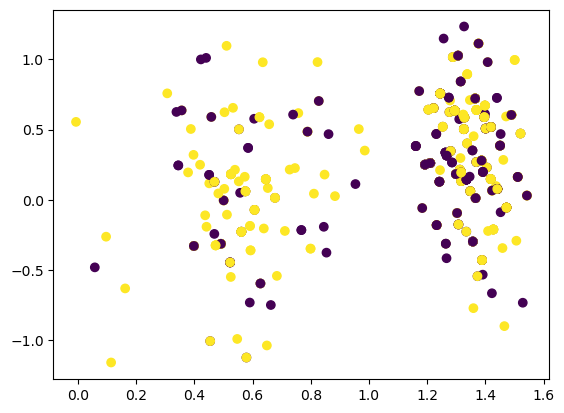
\includegraphics[width=0.35\textwidth]{figures/2dplot.png}
  \caption{Dimension reduction with 2 Principal Components}
  \label{fig:2PC}
\end{figure}

\begin{figure}[H]
  \centering
  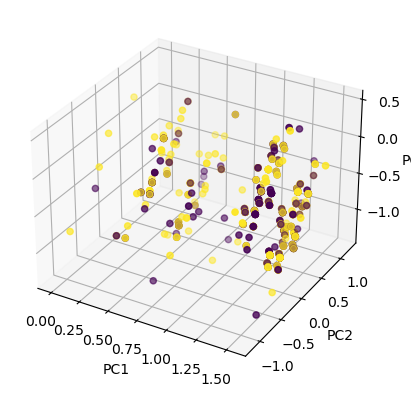
\includegraphics[width=0.35\textwidth]{figures/3dplot.png}
  \caption{Dimension reduction with 3 Principal Components}
  \label{fig:3PC}
\end{figure}
The final dataset had 686 examples and this was split into a training and testing set of size 548 and 138 respectively
\section{Methods}
\subsection{Evaluation}
We evaluate the models by calculating accuracy precision and recall.\\
Given the True Positives, False Positives, True Negatives and False Negatives of the predictions we have the following
\begin{align}
\text{Accuracy} &= \frac{TN + TP}{TN + FP + FN + TP} \\
\text{Precision} &= \frac{TP}{TP + FP} \\
\text{Recall} &= \frac{TP}{TP + FN}
\end{align}

\subsection{Logistic Regression}
The first model used is one of Logistic Regression fitted using Fisher Scoring. 
Fisher Scoring is the application of newton's method for finding the zero of a function to maximize the logistic regression log likelihood function.
It follows that since the maxima of the log likelihood function $\ell$ corresponds to points where it's first derivative is zero,
by finding the zero of the first derivative of the log likelihood $\ell'(\theta)$, we maximize the log likelihood. This gives the update rule
\begin{align*}
    \theta &:= \theta - \frac{\ell'(\theta)}{\ell''(\theta)}
\end{align*}
Note that the Hessian Matrix $H$ of a function is a matrix made up of the second-order partial derivatives of the function with
respect to it's inputs so we have $H = \ell''(\theta)$, also note that in logistic regression,
$\theta$ is vector valued. With these we get the update rule 
\begin{align*}
    \theta &:= \theta - H^{-1} \nabla_{\theta}\ell'(\theta)
\end{align*}

This is the update rule with which the model was fitted.
\subsection{Naive Bayes}
The second model used is a Naive Bayes model.\\
Naive Bayes is a Generative Learning Algorithm that derives the posterior distribution on y given x $P(y|x)$ using Bayes Rule. i.e
\begin{align*}
    P(y|x) &= \frac{P(x|y) \cdot P(y)}{P(x)}
\end{align*}
Naive Bayes also makes the wrong but useful assumption that all features are conditionally independent given their labels. i.e $P(x_j) = P(x_j| y, x_{j+i})$.
Furthermore $P(x)$ is ignored as it is a constant factor for all classes and does not affect the decision boundary.

Following these assumptions, we can expand Bayes Rule further to become:
\begin{align}
    P(y = 1|x) &= \prod_{j=1}^{d} p(x_j | y = 1) \cdot p(y=1)
\end{align}
Using the above, the probabilities $P(y = 1 | x)$ and $P(y = 0 | x)$ are calculated and the class with the highest probability is
chosen as our prediction.

To fit the model, we store the total counts where 
$x_j = 0 \land y = 1$,
$x_j = 1 \land y = 1$,
$x_j = 0 \land y = 0$ and 
$x_j = 1 \land y = 0$

Finally, to predict we use these stored counts to calculate the posterior distribution using the equation in 4
% \subsection{Decision Trees}
% The third model used is a Classification Decision Tree. 
% A Decision Tree is a non-parametric supervised learning method that uses \emph{split functions} to recursively partitions the problems feature space until max depth is reached. 

% To fit the model, we build the decision tree by first generating candidate split functions $\theta = (j, t)$ (where j is a feature and t is a threshold function).

% Next, we pick the split function that maximizes information gain. 
% Information gain is the difference between the mis-classification loss of the parent and the combined mis-classification loss across the children nodes that are created after the split.
% \begin{align*}
%     IG &= L(Q_p) - (L(Q_1) + L(Q_2))
% \end{align*}
% To calculate mis-classification loss we use the Cross Entropy Loss function. Because it is a concave function, by using it as our loss function we are guaranteed to get new information with every split
\subsection{Custom Generalized Linear Model}
Our label $y$, thus far has been whether our user with most ratings, Karen, likes a restaurant or not. 
For the sake of our custom GLM, we will instead predict the rating (1 - 5) the user would have given to the restaurant.

Generalized Linear Models are good at solving real life problems that can be modeled by probability distributions in the exponential family.

The response varibale is the rating the user would have given to the restaurant, because this response variable is continuous it can be modeled as a Gaussian Distribution.

The probability density function of the Gaussian Distribution is given by
\begin{align*}
  f(x) = \frac{1}{\sigma\sqrt{2\pi}} \exp\left(-\frac{1}{2} \left(\frac{(x - \mu)}{\sigma}\right)^2\right)
\end{align*}

Furthermore when constructing a GLM, we make the following assumptions

\begin{enumerate}
    \item $P(y|X; \theta)$ is modeled after the exponential family
    \item The models hypothesis function will be predicting $E[y|x]$
    \item the natural parameter $\eta$ and features X, are related linearly
\end{enumerate}

By modelling the users rating as a Gaussian Distribution, we have satisfied the first assumption.

From the second assumption, we see that $$h(X) = E[y|X] = \mu$$

From the third assumption, we know that the canonical parameter $\eta$ is linearly related to X

To identify the canonical parameter $\eta$, we write the probability density function of the Gaussian Distribution in exponential family form

\begin{align*}
  p(y; \eta, \tau) &= b(\alpha, \tau) \exp\left(\frac{\eta^T T(y) - a(\eta)}{c(\tau)}\right) \\
  p(y; \eta, \tau) &= b(\alpha, \tau) \exp\left(\frac{\eta^T T(y) - a(\eta)}{\sigma^2}\right) \\
  p(y ; \eta) &= \frac{1}{\sqrt{2\pi}} \exp\left(-\frac{1}{2}\left(\frac{y - \mu}{\sigma}\right)^2\right) \\
  &= \frac{1}{\sqrt{2\pi}} \exp\left(-\frac{1}{2}y^2\right) \exp\left( (x\eta - \frac{1}{2}\eta^2) T(y) \right)
\end{align*}



% There are 3 components of a Generalized Linear model
% \begin{enumerate}
%     \item Random Component
%     \item Systematic Component
%     \item Link
% \end{enumerate}

% The random component identifies the response variable and a probability distribution for it. 
% We know from assumption 1 above that $P(y |X; \theta)$ is modeled after the exponenetial family. this gives us
% \begin{align*}
%     p(y; \eta) \sim b(y) \exp(\eta^TT(y)-a(\eta))
% \end{align*}
% where $T(y)$ is the sufficient statistic for the distribution, $a(\eta)$ is the log partition function and $b(y)$ is the normalization constant. 
% The random component of our model is thus $p(y; \eta) \sim \mathcal{N}(\eta, \sigma^2)$, i.e modeled following the Gaussian Distribution


\section{Results and Discussion}

\end{document}
